%! Author = dmitriy
%! Date = 9/15/23

% Preamble
\documentclass[14pt]{extreport}
\usepackage{gost}
\usepackage{ragged2e}

%\usepackage{blindtext}
\justifying
\renewcommand{\thefigure}{\arabic{figure}}
\renewcommand{\thetable}{\arabic{table}}


\begin{document}
    \pagestyle{empty}
    
\includepdf[pages=-,pagecommand={}]{title.pdf}
    \pagestyle{plain}
    \tableofcontents

    \intro В данном отчете мы рассмотрим составление запросов на языке SQL (пункты 1-2) и оптимизацию их выполнения с использованием индексов. Для каждого запроса предложим соответствующие индексы, обоснуем выбор таблиц и атрибутов, а также опишем тип индекса. Далее рассмотрим возможные планы выполнения запросов без индексов и выберем оптимальный план. После добавления индексов рассмотрим, как изменяются выбранные планы выполнения запросов, предоставив вывод команды EXPLAIN ANALYZE для каждого запроса.

    \chapter{Текст задания:}
        \begin{figure}[h]
            \centering
            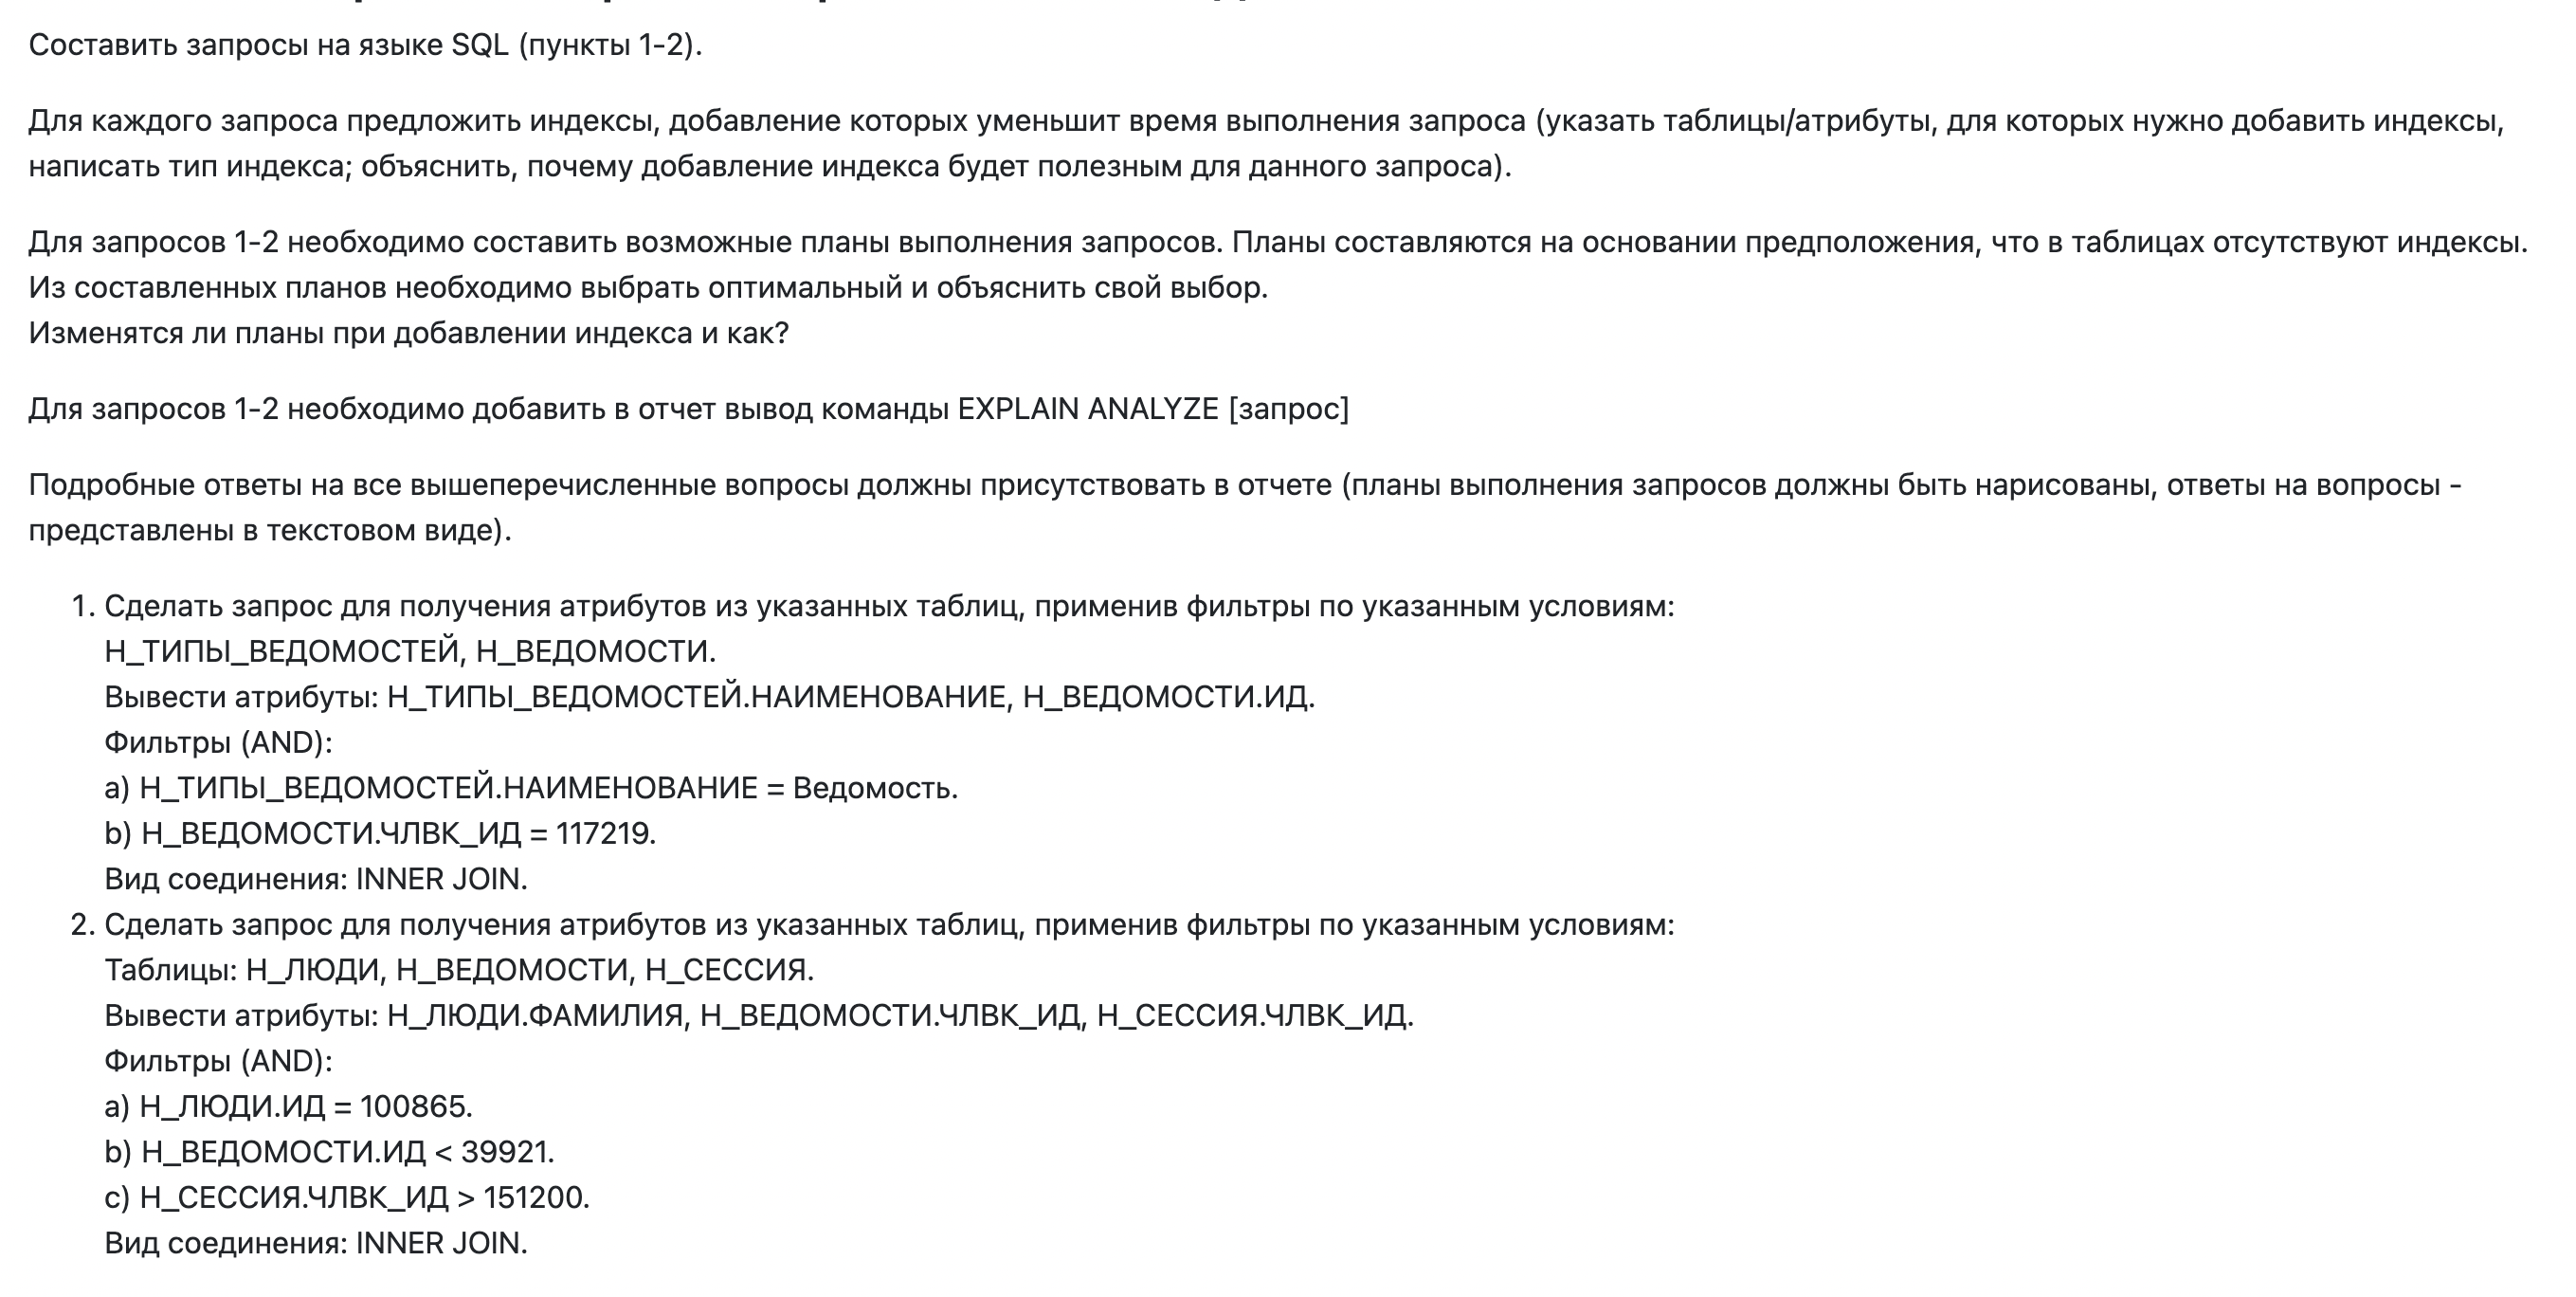
\includegraphics[width=0.99\textwidth]{task.png}
            \caption{Текст задания}
        \end{figure}

    \chapter{Запросы:}
    \begin{verbatim}
-- 1 Запрос
SELECT Н_ТИПЫ_ВЕДОМОСТЕЙ.НАИМЕНОВАНИЕ, Н_ВЕДОМОСТИ.ИД
FROM Н_ТИПЫ_ВЕДОМОСТЕЙ
         INNER JOIN Н_ВЕДОМОСТИ ON Н_ТИПЫ_ВЕДОМОСТЕЙ.ИД = Н_ВЕДОМОСТИ.ТВ_ИД
WHERE Н_ТИПЫ_ВЕДОМОСТЕЙ.НАИМЕНОВАНИЕ = 'Ведомость'
  AND Н_ВЕДОМОСТИ.ЧЛВК_ИД = 117219;

-- 2 Запрос
SELECT Н_ЛЮДИ.ФАМИЛИЯ, Н_ВЕДОМОСТИ.ЧЛВК_ИД, Н_СЕССИЯ.ЧЛВК_ИД
FROM Н_ЛЮДИ
         INNER JOIN Н_ВЕДОМОСТИ ON Н_ЛЮДИ.ИД = Н_ВЕДОМОСТИ.ЧЛВК_ИД
         INNER JOIN Н_СЕССИЯ ON Н_ВЕДОМОСТИ.ЧЛВК_ИД = Н_СЕССИЯ.ЧЛВК_ИД
WHERE Н_ЛЮДИ.ИД = 100865
  AND Н_ВЕДОМОСТИ.ИД < 39921
  AND Н_СЕССИЯ.ЧЛВК_ИД > 151200;
    \end{verbatim}

\chapter{Индексы}

        \section*{Запрос 1:}

            \subsection*{Таблица \texttt{Н\_ТИПЫ\_ВЕДОМОСТЕЙ}:}
                \begin{itemize}
                    \item Индекс по столбцу \texttt{НАИМЕНОВАНИЕ} с типом \texttt{B-Tree}.
                    \begin{itemize}
                        \item \textbf{Объяснение:} Этот индекс ускорит поиск записей по наименованию типа ведомости.
                    \end{itemize}
                \end{itemize}

            \subsection*{Таблица \texttt{Н\_ВЕДОМОСТИ}:}
                \begin{itemize}
                    \item Индекс по столбцам \texttt{ТВ\_ИД} и \texttt{ЧЛВК\_ИД} с типом \texttt{B-Tree}.
                    \begin{itemize}
                        \item \textbf{Объяснение:} Данный составной индекс улучшит производительность запроса, который использует условия фильтрации и соединение по этим двум столбцам.
                    \end{itemize}
                \end{itemize}

        \section*{Запрос 2:}

            \subsection*{Таблица \texttt{Н\_ЛЮДИ}:}
                \begin{itemize}
                    \item Индекс по столбцу \texttt{ИД} с типом \texttt{B-Tree}.
                    \begin{itemize}
                        \item \textbf{Объяснение:} Этот индекс ускорит поиск записей по идентификатору человека.
                    \end{itemize}
                \end{itemize}

            \subsection*{Таблица \texttt{Н\_ВЕДОМОСТИ}:}
                \begin{itemize}
                    \item Индекс по столбцам \texttt{ЧЛВК\_ИД} и \texttt{ИД} с типом \texttt{B-Tree}.
                    \begin{itemize}
                        \item \textbf{Объяснение:} Составной индекс улучшит условие соединения с таблицей \texttt{Н\_СЕССИЯ} и условие по столбцу \texttt{ИД}.
                    \end{itemize}
                \end{itemize}

            \subsection*{Таблица \texttt{Н\_СЕССИЯ}:}
                \begin{itemize}
                    \item Индекс по столбцу \texttt{ЧЛВК\_ИД} с типом \texttt{B-Tree}.
                    \begin{itemize}
                        \item \textbf{Объяснение:} Этот индекс ускорит поиск записей по идентификатору человека в таблице сессий.
                    \end{itemize}
                \end{itemize}

\chapter{Планы запросов:}
        \section*{Запрос 1:}

            \subsection*{Возможные планы выполнения без индексов:}

                1. \textbf{План №1 (Nested Loop Join):}
                \begin{itemize}
                    \item Поиск записи в таблице \texttt{Н\_ТИПЫ\_ВЕДОМОСТЕЙ} по условию \texttt{НАИМЕНОВАНИЕ = 'Ведомость'}.
                    \item Для каждой найденной записи выполняется поиск соответствующей записи в таблице \texttt{Н\_ВЕДОМОСТИ} по условию \texttt{ТВ\_ИД = ИД найденной записи}.
                \end{itemize}
                \begin{verbatim}
Nested Loop Join
|-- Scan ТИПЫ_ВЕДОМОСТЕЙ
|   `-- Filter: (НАИМЕНОВАНИЕ = 'Ведомость')
`-- Scan по ВЕДОМОСТИ
    `-- Condition: (ТВ_ИД = ТИПЫ_ВЕДОМОСТЕЙ.ИД)
        `-- Filter: (ЧЛВК_ИД = 117219)
                \end{verbatim}


                2. \textbf{План №2 (Hash Join):}
                \begin{itemize}
                    \item Полное сканирование обеих таблиц, фильтрация записей по условиям, а затем объединение результатов.
                \end{itemize}
                \begin{verbatim}
Hash Join
|-- Scan ВЕДОМОСТИ
|   `-- Filter: (ЧЛВК_ИД = 117219)
`-- Hash
    |-- Scan ТИПЫ_ВЕДОМОСТЕЙ
    |   `-- Filter: (НАИМЕНОВАНИЕ = 'Ведомость')
    `-- Condition: (ВЕДОМОСТИ.ТВ_ИД = ТИПЫ_ВЕДОМОСТЕЙ.ИД)
                \end{verbatim}


                \subsubsection*{Оптимальный план:}
                    План №1 (Nested Loop Join) - Объяснение: В данном случае, так как у нас есть точные условия для выборки по индексам, использование вложенного цикла (Nested Loop Join) с фильтрацией по индексу в таблице \texttt{Н\_ТИПЫ\_ВЕДОМОСТЕЙ} и \texttt{Н\_ВЕДОМОСТИ} будет наиболее эффективным.

                    \begin{figure}[h]
                            \centering
                            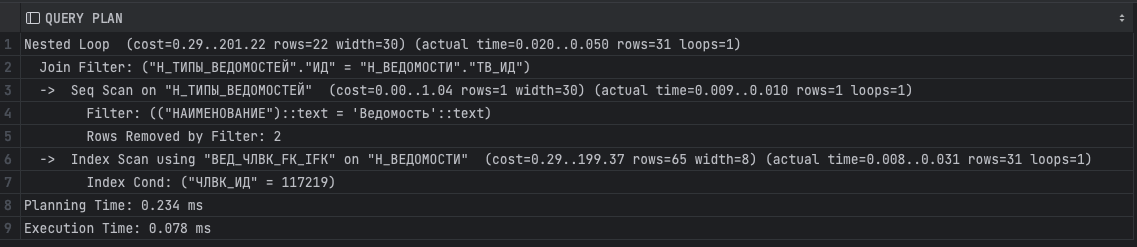
\includegraphics[width=0.99\textwidth]{q1.png}
                            \caption{EXPLAIN ANALYZE}
                    \end{figure}


                \subsubsection*{Изменение планов при добавлении индексов:}
                    Добавление индексов улучшит эффективность выполнения обоих планов. В частности, появятся возможности для использования индексных операций, таких как Index Scan или Index Nested Loop Join, что существенно снизит количество записей, которые необходимо просмотреть для выполнения запроса.



        \section*{Запрос 2:}

            \subsection*{Возможные планы выполнения без индексов:}

                1. \textbf{План №1 (Nested Loop Join):}
                \begin{itemize}
                    \item Поиск записи в таблице \texttt{Н\_ЛЮДИ} по условию \texttt{ИД = 100865}.
                    \item Для каждой найденной записи выполняется поиск соответствующей записи в таблице \texttt{Н\_ВЕДОМОСТИ} по условию \texttt{ЧЛВК\_ИД = ИД найденной записи}.
                    \item Затем для каждой записи из \texttt{Н\_ВЕДОМОСТИ} выполняется поиск соответствующей записи в таблице \texttt{Н\_СЕССИЯ} по условию \texttt{ЧЛВК\_ИД = ИД найденной записи}.
                \end{itemize}
                \begin{verbatim}
Nested Loop Join
|-- Scan по ЛЮДИ
|   `-- Сondition: (ИД = 100865)
`-- Nested Loop Join
    |-- Scan по ВЕДОМОСТИ
    |   |-- Condition: (ЧЛВК_ИД = 100865)
    |   `-- Filter: (ИД < 39921)
    `-- Scan по СЕССИЯ
        |-- Condition: (ЧЛВК_ИД = 100865)
        `-- Filter: (ЧЛВК_ИД > 151200)
                \end{verbatim}

                2. \textbf{План №2 (Hash Join):}
                \begin{itemize}
                    \item Полное сканирование всех трех таблиц, фильтрация записей по условиям, а затем объединение результатов.
                \end{itemize}
                \begin{verbatim}
Hash Join
|-- Scan СЕССИЯ
|   `-- Filter: (ЧЛВК_ИД > 151200)
`-- Hash
    |-- Nested Loop
    |   |-- Scan по ЛЮДИ
    |   |   `-- Condition: (ИД = 100865)
    |   `-- Scan по ВЕДОМОСТИ
    |       |-- Condition: (ЧЛВК_ИД = 100865)
    |       `-- Filter: (ИД < 39921)
    `-- Condition: (СЕССИЯ.ЧЛВК_ИД = ВЕДОМОСТИ.ЧЛВК_ИД)
                \end{verbatim}


                \begin{figure}[h]
                    \centering
                    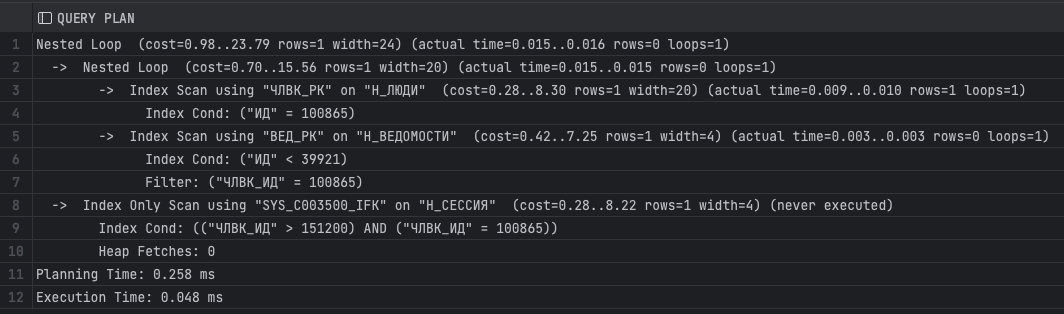
\includegraphics[width=0.99\textwidth]{q2.png}
                    \caption{EXPLAIN ANALYZE}
                \end{figure}

                \subsubsection*{Оптимальный план:}
                    План №1 (Nested Loop Join) - Объяснение: В данном случае, так как у нас есть точные условия для выборки по индексам, использование вложенного цикла (Nested Loop Join) с фильтрацией по индексу в таблице \texttt{Н\_ЛЮДИ} и последующими объединениями с таблицами \texttt{Н\_ВЕДОМОСТИ} и \texttt{Н\_СЕССИЯ} будет наиболее эффективным.

                \subsubsection*{Изменение планов при добавлении индексов:}
                    Добавление индексов улучшит эффективность выполнения обоих планов, особенно при использовании Index Scan или Index Nested Loop Join. Индексы на столбцы, используемые в условиях фильтрации и соединения, существенно сократят количество записей, которые необходимо просмотреть.

                \conclusions В ходе лабораторной работы были рассмотрены два SQL-запроса с указанием возможных планов выполнения без индексов. Для каждого запроса был выбран оптимальный план, основанный на предположении отсутствия индексов. В контексте оптимизации производительности были предложены индексы для соответствующих таблиц и атрибутов, что должно значительно снизить время выполнения запросов. При добавлении индексов предполагается улучшение эффективности выполнения запросов за счет оптимизированных операций поиска и объединения данных.
\end{document}